\documentclass[11pt]{article}

\usepackage[utf8]{inputenc}
\usepackage[T1]{fontenc}
\usepackage{lmodern}
\usepackage{geometry}
\geometry{margin=1in}
\usepackage{graphicx}
\usepackage{booktabs}
\usepackage{tabularx}
\usepackage{array}
\usepackage{amsmath}
\usepackage{amssymb}
\usepackage{float}
\usepackage{microtype}
\usepackage[numbers,sort&compress]{natbib}
\usepackage{xcolor}
\usepackage[font=small,labelfont=bf]{caption}
\usepackage{hyperref}
\definecolor{linkblue}{HTML}{1F4E79}
\definecolor{urlteal}{HTML}{0B6E6E}
\hypersetup{
  colorlinks=true,
  linkcolor=linkblue,
  citecolor=linkblue,
  urlcolor=urlteal,
  pdftitle={A Psychometric Audit of Open LLM Benchmarks: Capacity-Conditioned Alignment Tax in 591 Architectures},
  pdfauthor={Preston Botter}
}
\urlstyle{same}
\newcolumntype{Y}{>{\raggedright\arraybackslash}X}

\title{\textbf{A Psychometric Audit of Open LLM Benchmarks: Capacity-Conditioned Alignment Tax in 591 Architectures}}
\author{Preston Botter\\Ph.D. Student, Indiana University Bloomington\\\texttt{pbotter@iu.edu}}
\date{April 23, 2026}

\begin{document}
\maketitle

\begin{abstract}
Leaderboard rank is often treated as a direct proxy for broad model ability, but psychometric theory suggests that high scores and coherent latent structure are not identical. This paper presents a psychometric audit of 591 deduplicated open-weight LLM architectures and 12,061 binary items from the April 8, 2024 Open LLM Leaderboard snapshot. We define the latent-structure alignment tax as an ability-conditioned deterioration in shared factor structure, measured with leave-one-out jackknife concentration shift ($\Delta g$), and ask whether that deterioration rises monotonically with ability. The audited matrix retains a dominant first factor (PC1 variance explained $=36.26\%$), and ability is reported on a standardized $g$ scale (mean 0, SD 1). Descriptively, ability and structural impact are positively associated, but the full relation is strongly nonlinear. Quadratic influence models and decile summaries show an inverted-U pattern: structural pollution peaks in a middle-ability band and attenuates in the upper tail. We therefore interpret the latent-structure alignment tax in this snapshot as a capacity-conditioned bifurcation rather than a uniform degradation law. Family-level summaries for Llama, Mistral/Mixtral, Qwen, Gemma, and DeepSeek are consistent with this interpretation and show substantial within-family heterogeneity, most clearly in Llama.
\end{abstract}

\section{Introduction}
The main measurement problem in contemporary LLM evaluation is not whether models can improve, but what exactly a reported improvement means. Benchmark optimization can raise aggregate scores while simultaneously changing what those scores represent. In that sense, current evaluation practice sits squarely in a Goodhart setting \citep{goodhart1975problems, strathern1997improving}: once a proxy metric is directly optimized as a target, its statistical relation to the underlying construct can degrade. Recent benchmarking work documents contamination risk, benchmark aging, and protocol sensitivity, all of which complicate score interpretation \citep{liang2023helm, kiela2021dynabench, wu2025antileakbench, chen2025emnlpcontam, alzahrani2024targets}.

This motivates our use of the term \emph{latent-structure (psychometric) alignment tax}: benchmark-oriented optimization can improve observed aggregate performance while degrading latent construct structure at a fixed ability level \citep{federiakin2025leaderboards, zhou2026lost, li2026adaptive}. In this manuscript, the term is operational and geometric, not rhetorical. It refers to jackknife-detected structural degradation conditional on standardized ability.

Psychometric $g$ research provides a useful framing for this issue. In the classical tradition, $g$ is inferred from a positive manifold across tasks rather than read off any single observed score \citep{spearman1904general, carroll1993human, jensen1998g}. That distinction matters for LLMs: two systems can have similar leaderboard totals while occupying different positions in latent-structure space.

Related work on LLM evaluation already points in this direction. Factor-analytic studies find a strong common dimension, but not a single undifferentiated performance surface \citep{burnell2023structure, ilic2024interrelated}. IRT-style and adaptive evaluation papers reach a similar conclusion from the item side: item difficulty, discrimination, and item selection materially affect how model ability is estimated and compared \citep{zhou2026lost, tambon2025taskeval, taschetto2025enem, truong2025amortized, li2026adaptive, liao2025legoirt}. Recent benchmark research also emphasizes rank instability, contamination sensitivity, and the need for psychometrically grounded comparisons rather than raw score averages \citep{federiakin2025leaderboards, wu2025antileakbench, chen2025emnlpcontam, chen2025recentcontam}.

In this manuscript, the latent-structure alignment tax is operationalized with a single structural measure, jackknife concentration shift ($\Delta g$), which quantifies how much each model perturbs first-factor concentration in leave-one-out analyses.

The present study asks a targeted question: once ability and latent-structure impact are measured separately, is structural pollution a monotonic function of ability or a bifurcating one? To answer this, we conduct an item-level audit of open models, estimate leave-one-out structural influence, and fit nonlinear influence surfaces under explicit uncertainty quantification.

\section{Data}
Let $X \in \{0,1\}^{n \times p}$ denote the model-by-item response matrix, where $n=591$ and $p=12{,}061$. Rows correspond to deduplicated model architectures. The dataset is a fixed historical slice (April 8, 2024) and intentionally excludes post-snapshot models.

Item-level responses are taken from the Open LLM Leaderboard release \citep{openllmleaderboard2024}. Architecture filtering and deduplication follow the workflow reported by \citet{ilic2024interrelated}. Data and code for this audit are available at \url{https://github.com/pbotter42/LLMbench}.

Define $\mu \in \mathbb{R}^{p}$ as the itemwise mean and the centered matrix
\[
X_c = X - \mathbf{1}\mu^\top.
\]
All results in this manuscript are computed from this fixed matrix with bootstrap uncertainty where appropriate.

\subsection{Software Environment}
All analyses were executed in R (version 4.4.0). Compute was performed on a MacBook Air (Apple M2, 8 GB memory, macOS 15.7.3). Reproducible code and workflow materials are available at \url{https://github.com/pbotter42/LLMbench}.

\section{Mathematical Framework}
\subsection{Ability as the First Principal Component}
We compute the singular value decomposition
\[
X_c = UDV^\top,
\]
where $D=\mathrm{diag}(d_1,\ldots,d_r)$ with $d_1 \ge d_2 \ge \cdots$. The first loading vector is $v_1 = V_{\cdot 1}$, and the oriented raw PC1 ability score for model $i$ is
\[
a_i = s\,(U_{i1}d_1),
\]
with orientation sign $s \in \{-1,1\}$ chosen so that larger values align with larger external ability metadata when available. For reporting and regression we use standardized ability,
\[
g_i = \frac{a_i-\bar a}{s_a},
\]
where $\bar a$ and $s_a$ are the sample mean and standard deviation of $\{a_i\}_{i=1}^n$. The fraction of variance explained by PC1 is
\[
\pi_1 = \frac{d_1^2}{\sum_{k=1}^{r} d_k^2}.
\]

\subsection{Structural Influence by Jackknife}
For each model $i$, recompute PCA on $X_{-i}$ (row $i$ removed) and define
\[
\Delta g_i = \pi_1^{(-i)} - \pi_1.
\]
Interpretation is direct: $\Delta g_i>0$ means removing model $i$ increases first-factor concentration (polluter), while $\Delta g_i<0$ means removing model $i$ decreases concentration (pillar).

\subsection{Nonlinear Fracture Model and Uncertainty}
To test monotonic versus bifurcating fracture, we estimate
\[
\Delta g_i = \beta_0 + \beta_1 g_i + \beta_2 g_i^2 + \beta_3 \log(1+\mathrm{params}_i) + \gamma^\top t_i + \varepsilon_i,
\]
where $t_i$ are model-type indicators from conservative name-based parsing, and $g_i$ is standardized ability (mean 0, SD 1). The key test is $H_0:\beta_2=0$. We compare linear and quadratic models by nested ANOVA and compute nonparametric bootstrap percentile confidence intervals ($B=10{,}000$) \citep{efron1979bootstrap}.

\subsection{Regression Specifications and Rationale}
Three regression specifications are estimated for $\Delta g$:
\[
\text{M1: }\Delta g_i=\beta_0+\beta_1 g_i+\varepsilon_i,
\]
\[
\text{M2: }\Delta g_i=\beta_0+\beta_1 g_i+\beta_2 g_i^2+\varepsilon_i,
\]
\[
\text{M3: }\Delta g_i=\beta_0+\beta_1 g_i+\beta_2 g_i^2+\beta_3\log(1+\mathrm{params}_i)+\gamma^\top t_i+\varepsilon_i.
\]
M1 is a monotonic baseline, M2 is the fracture model used to test curvature ($\beta_2\neq 0$), and M3 tests whether the M2 shape persists after size and model-type controls. Bootstrap percentile intervals ($B=10{,}000$) are reported for all model $R^2$ values and for the M2 turning point $g^\star$.

\begin{table}[H]
\centering
\small
\begin{tabularx}{\textwidth}{@{}l>{\raggedright\arraybackslash}p{0.44\textwidth}Y@{}}
\toprule
Model & Regression form & Purpose \\
\midrule
M1 & $\Delta g\sim g$ & Linear baseline for monotonic structural change \\
M2 & $\Delta g\sim g+g^2$ & Quadratic test for a middle-band peak in structural impact \\
M3 & $\Delta g\sim g+g^2+\log(1+\mathrm{params})+\mathrm{type}$ & Quadratic model with parameter-count and type controls \\
\bottomrule
\end{tabularx}
\caption{Regression models used in the analysis and their inferential role.}
\label{tab:reg_models_method}
\end{table}

\subsection{Formal Definition of Capacity-Conditioned Bifurcation}
Let
\[
m(g)=\mathbb{E}[\Delta g\mid g]
\]
be the conditional mean structural impact at ability level $g$. A monotonic-fracture model would require $m'(g)\ge 0$ over the observed ability range. In contrast, capacity-conditioned bifurcation is defined by the existence of a turning point $g^\star$ such that
\[
m'(g)>0\ \text{for}\ g<g^\star,\qquad
m'(g)<0\ \text{for}\ g>g^\star,
\]
with $m(g)$ positive in a middle interval and near-zero or negative in at least one tail interval. In this study, $m(g)$ is estimated by the quadratic regression surface, so $g^\star=-\beta_1/(2\beta_2)$ when $\beta_2<0$.

\section{Results}
\subsection{Replication of the Dominant General Factor}
At item level, the audited snapshot still exhibits a pronounced common dimension: $\pi_1=0.3626$ (36.26\%). Figure~\ref{fig:scree} shows the familiar steep drop after the first component, which is exactly what one would expect if a strong shared factor remains present. The value may appear lower than estimates reported for benchmark-level aggregates, but that gap is expected rather than problematic. Item matrices retain item-specific variance that benchmark averages smooth away, so direct numerical agreement should not be expected \citep{burnell2023structure, ilic2024interrelated}.

\begin{figure}[H]
  \centering
  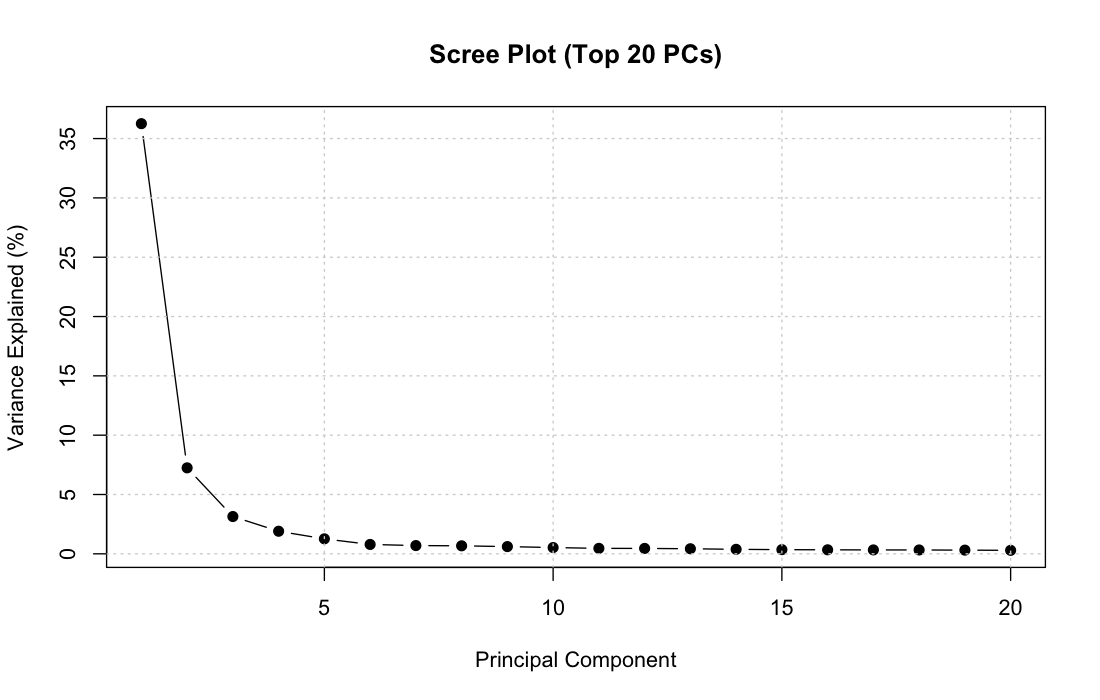
\includegraphics[width=0.74\textwidth]{../outputs/figure_scree_top20.png}
  \caption{Top-20 scree profile for the audited 591-model by 12,061-item matrix. The sharp drop after PC1 is consistent with a dominant common factor.}
  \label{fig:scree}
\end{figure}

Tables~\ref{tab:top10g} and \ref{tab:bottom10g} anchor the standardized ability scale by listing the top 10 and bottom 10 models on $g$. They make the range of the audit concrete before turning to the main structural result.

\begin{table}[H]
\centering
\scriptsize
\begin{tabular}{@{}p{0.68\textwidth}rr@{}}
\toprule
Model & $g$ & $\Delta g$ \\
\midrule
alchemonaut/QuartetAnemoi-70B-t0.0001 & 1.12 & $-0.00014$ \\
lodrick-the-lafted/Grafted-Llama2-2x70B & 1.11 & $-0.00017$ \\
cloudyu/Mixtral\_7Bx5\_MoE\_30B & 1.10 & $-0.00015$ \\
eldogbbhed/NeuralMonarchCoderPearlBeagle & 1.10 & $-0.00015$ \\
Sao10K/WinterGoddess-1.4x-70B-L2 & 1.10 & $-0.00015$ \\
Weyaxi/OpenHermes-2.5-neural-chat-v3-3-openchat-3.5-1210-Slerp & 1.09 & $-0.00014$ \\
ignos/LeoScorpius-GreenNode-Platypus-7B-v1 & 1.08 & $-0.00017$ \\
Steelskull/Umbra-MoE-4x10.7 & 1.08 & $-0.00012$ \\
jsfs11/SnorkelWestBeagle-DARETIES-7B & 1.08 & $-0.00013$ \\
PulsarAI/MetaMath-Chupacabra-7B-v2.01-Slerp & 1.08 & $-0.00017$ \\
\bottomrule
\end{tabular}
\caption{Top 10 models by standardized ability ($g$), shown as high-end anchors for the audited scale.}
\label{tab:top10g}
\end{table}

\begin{table}[H]
\centering
\scriptsize
\begin{tabular}{@{}p{0.68\textwidth}rr@{}}
\toprule
Model & $g$ & $\Delta g$ \\
\midrule
cerebras/Cerebras-GPT-111M & -2.05 & $-0.00120$ \\
Corianas/111m & -2.05 & $-0.00118$ \\
BEE-spoke-data/Mixtral-GQA-400m-v2 & -2.02 & $-0.00115$ \\
postbot/distilgpt2-emailgen & -2.02 & $-0.00114$ \\
euclaise/gpt-neox-122m-minipile-digits & -2.02 & $-0.00112$ \\
Felladrin/Minueza-32M-Chat & -2.02 & $-0.00108$ \\
BEE-spoke-data/verysmol\_llama-v11-KIx2 & -2.01 & $-0.00113$ \\
HWERI/pythia-70m-deduped-cleansharegpt-en & -2.00 & $-0.00107$ \\
Josephgflowers/distillgpt2Cinder & -2.00 & $-0.00107$ \\
ethzanalytics/pythia-31m & -2.00 & $-0.00104$ \\
\bottomrule
\end{tabular}
\caption{Bottom 10 models by standardized ability ($g$), shown as low-end anchors for the audited scale.}
\label{tab:bottom10g}
\end{table}

Several widely discussed checkpoints make the scale easier to read. Grafted-Llama2-2x70B ($g=1.11$, $\Delta g=-0.00017$), Qwen2-beta-72B ($g=1.01$, $\Delta g=-0.00005$), and a representative Mistral-7B-Instruct variant ($g=0.95$, $\Delta g=-0.00007$) sit in the high-ability, near-neutral to pillar region. By contrast, Gemma-7B-IT ($g=0.21$, $\Delta g=0.00050$) and DeepSeek-Coder-6.7B-Instruct ($g=-0.71$, $\Delta g=0.00041$) fall in the positive-impact polluter region for this snapshot.

\subsection{Ability--Impact Association}
As a descriptive summary, the bivariate relation between standardized ability and jackknife structural impact is positive:
\[
\mathrm{corr}(g,\Delta g)=0.542.
\]
Bootstrap 95\% confidence intervals place this correlation in
\[
[0.471,\,0.601],
\]
which excludes zero. Figure~\ref{fig:corr_gdelta} visualizes this association with a scatterplot and linear fit. The figure is useful mainly as a first-pass view of the data: the overall slope is clearly positive, but the point cloud also shows visible curvature. In other words, the marginal association is real, yet it already hints that a simple monotonic account is incomplete.

\begin{figure}[H]
  \centering
  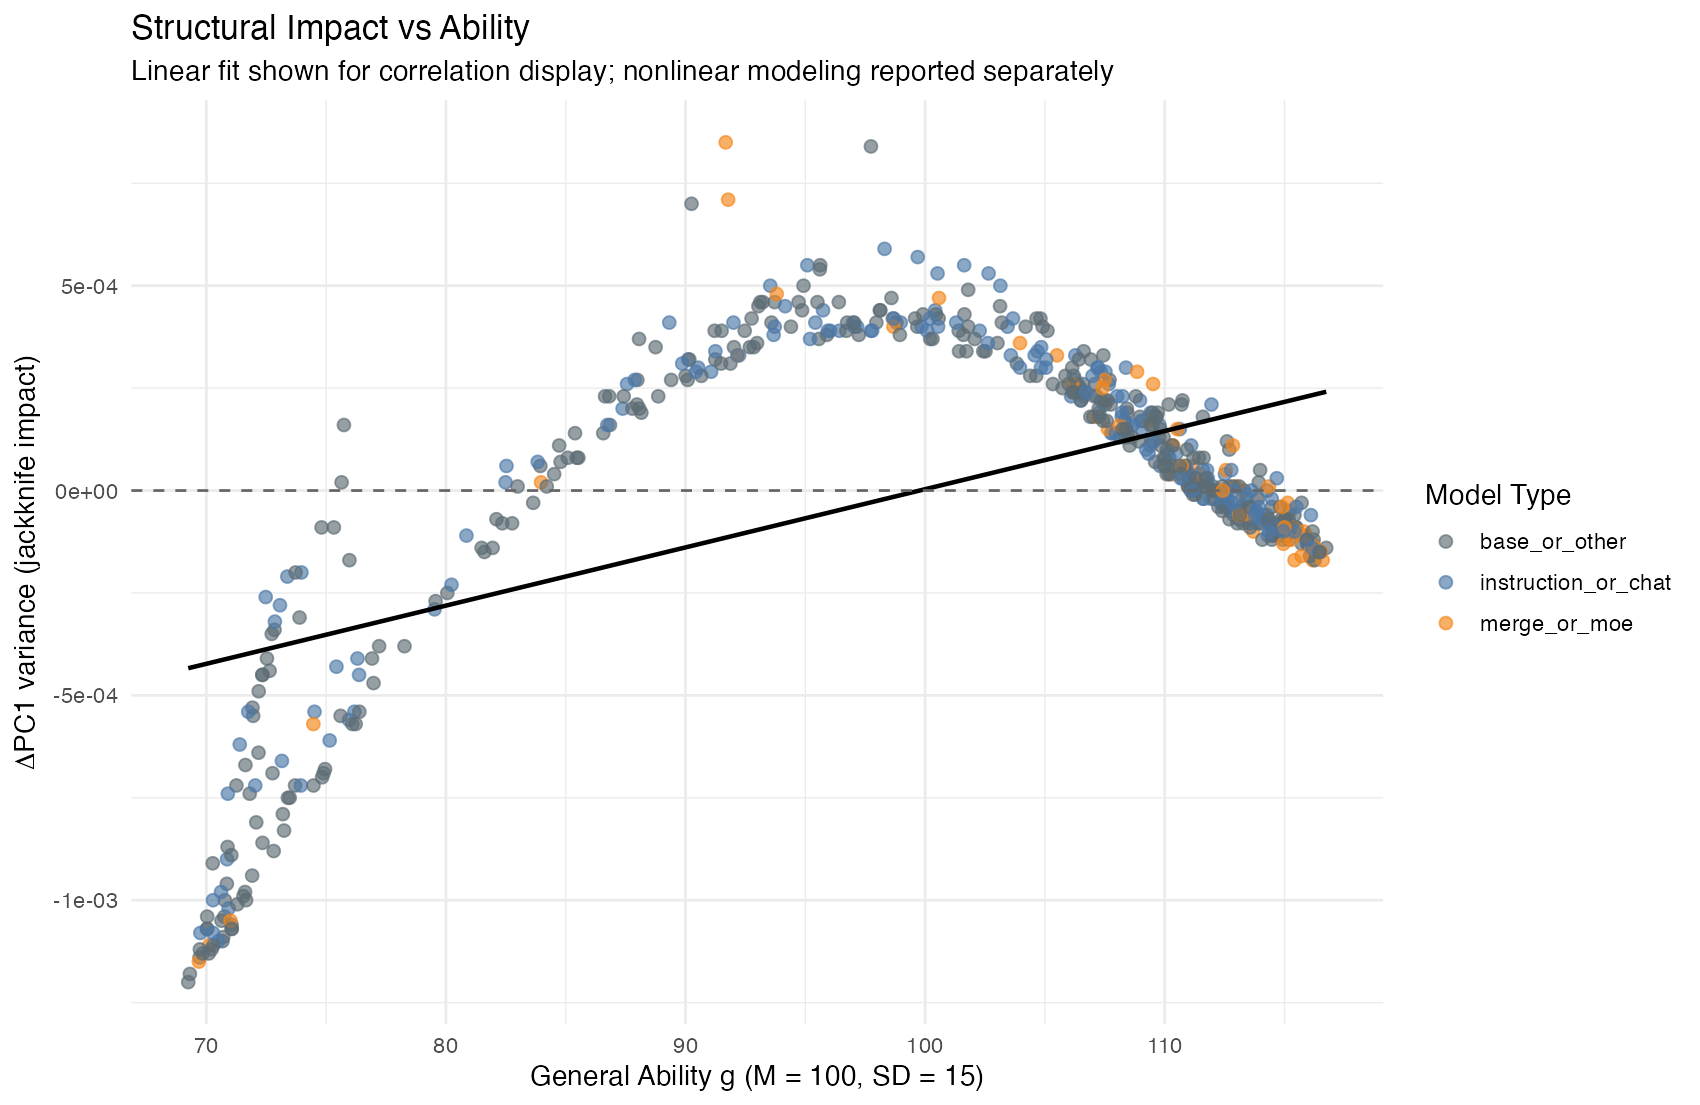
\includegraphics[width=0.94\textwidth]{../outputs/figure_ability_vs_delta.png}
  \caption{Ability and jackknife structural impact under a linear descriptive overlay. The positive slope captures the overall association, but not the curvature shown more directly in Figure~\ref{fig:middle_fracture}.}
  \label{fig:corr_gdelta}
\end{figure}

\subsection{Middle Fracture}
That nonlinearity becomes decisive once curvature is modeled. Using the model definitions in Table~\ref{tab:reg_models_method}, M1 (linear baseline) yields $R^2=0.294$ with bootstrap 95\% CI $[0.222,0.362]$. M2 (quadratic fracture) yields $R^2=0.927$ with bootstrap 95\% CI $[0.908,0.945]$. M3 (controlled quadratic) yields $R^2=0.933$ with bootstrap 95\% CI $[0.915,0.949]$. The M1--M2 nested comparison decisively favors curvature (ANOVA $p<.001$). The jump from M1 to M2 is the main empirical result of the paper: a forced linear story captures only a minority of the variation, whereas a quadratic surface captures nearly all of it. Decile summaries tell the same story in a model-free way, with mean $\Delta g$ negative in the lowest and highest ability deciles and maximal in the middle deciles. The empirical shape is therefore an inverted U, not a monotonic increase in pollution with ability.

The estimated quadratic relation is
\[
\widehat{\Delta g}
= 0.00041248
- 0.00012850\,g
- 0.00040991\,g^2.
\]
Both M2 slope coefficients are far from zero ($p<.001$ for both the linear and quadratic terms). The implied turning point is
\[
g^\star = -\frac{\hat{\beta}_1}{2\hat{\beta}_2}\approx -0.157,
\]
with peak predicted pollution $\widehat{\Delta g}(g^\star)\approx 0.000423$. Bootstrap uncertainty for these nonlinear functionals is narrow: $g^\star\in[-0.170,-0.144]$ and $\widehat{\Delta g}(g^\star)\in[0.0004105,0.0004355]$ (95\%).

The same turning-point structure appears in grouped summaries. In the lowest decile (\(g\in[-2.05,-1.81]\)), mean impact is \(-0.000878\) with 95\% CI \([-0.000944,-0.000813]\). In a middle decile (decile 4; \(g\in[-0.42,0.09]\)), mean impact rises to \(0.000435\) with 95\% CI \([0.000415,0.000454]\). In the upper tail (decile 10; \(g\in[0.98,1.12]\)), mean impact returns negative at \(-0.000105\) with 95\% CI \([-0.000115,-0.000094]\).

Figure~\ref{fig:middle_fracture} brings these pieces together directly: raw model points, a quadratic fit, and decile means aligned with the middle-band peak.

\begin{figure}[H]
  \centering
  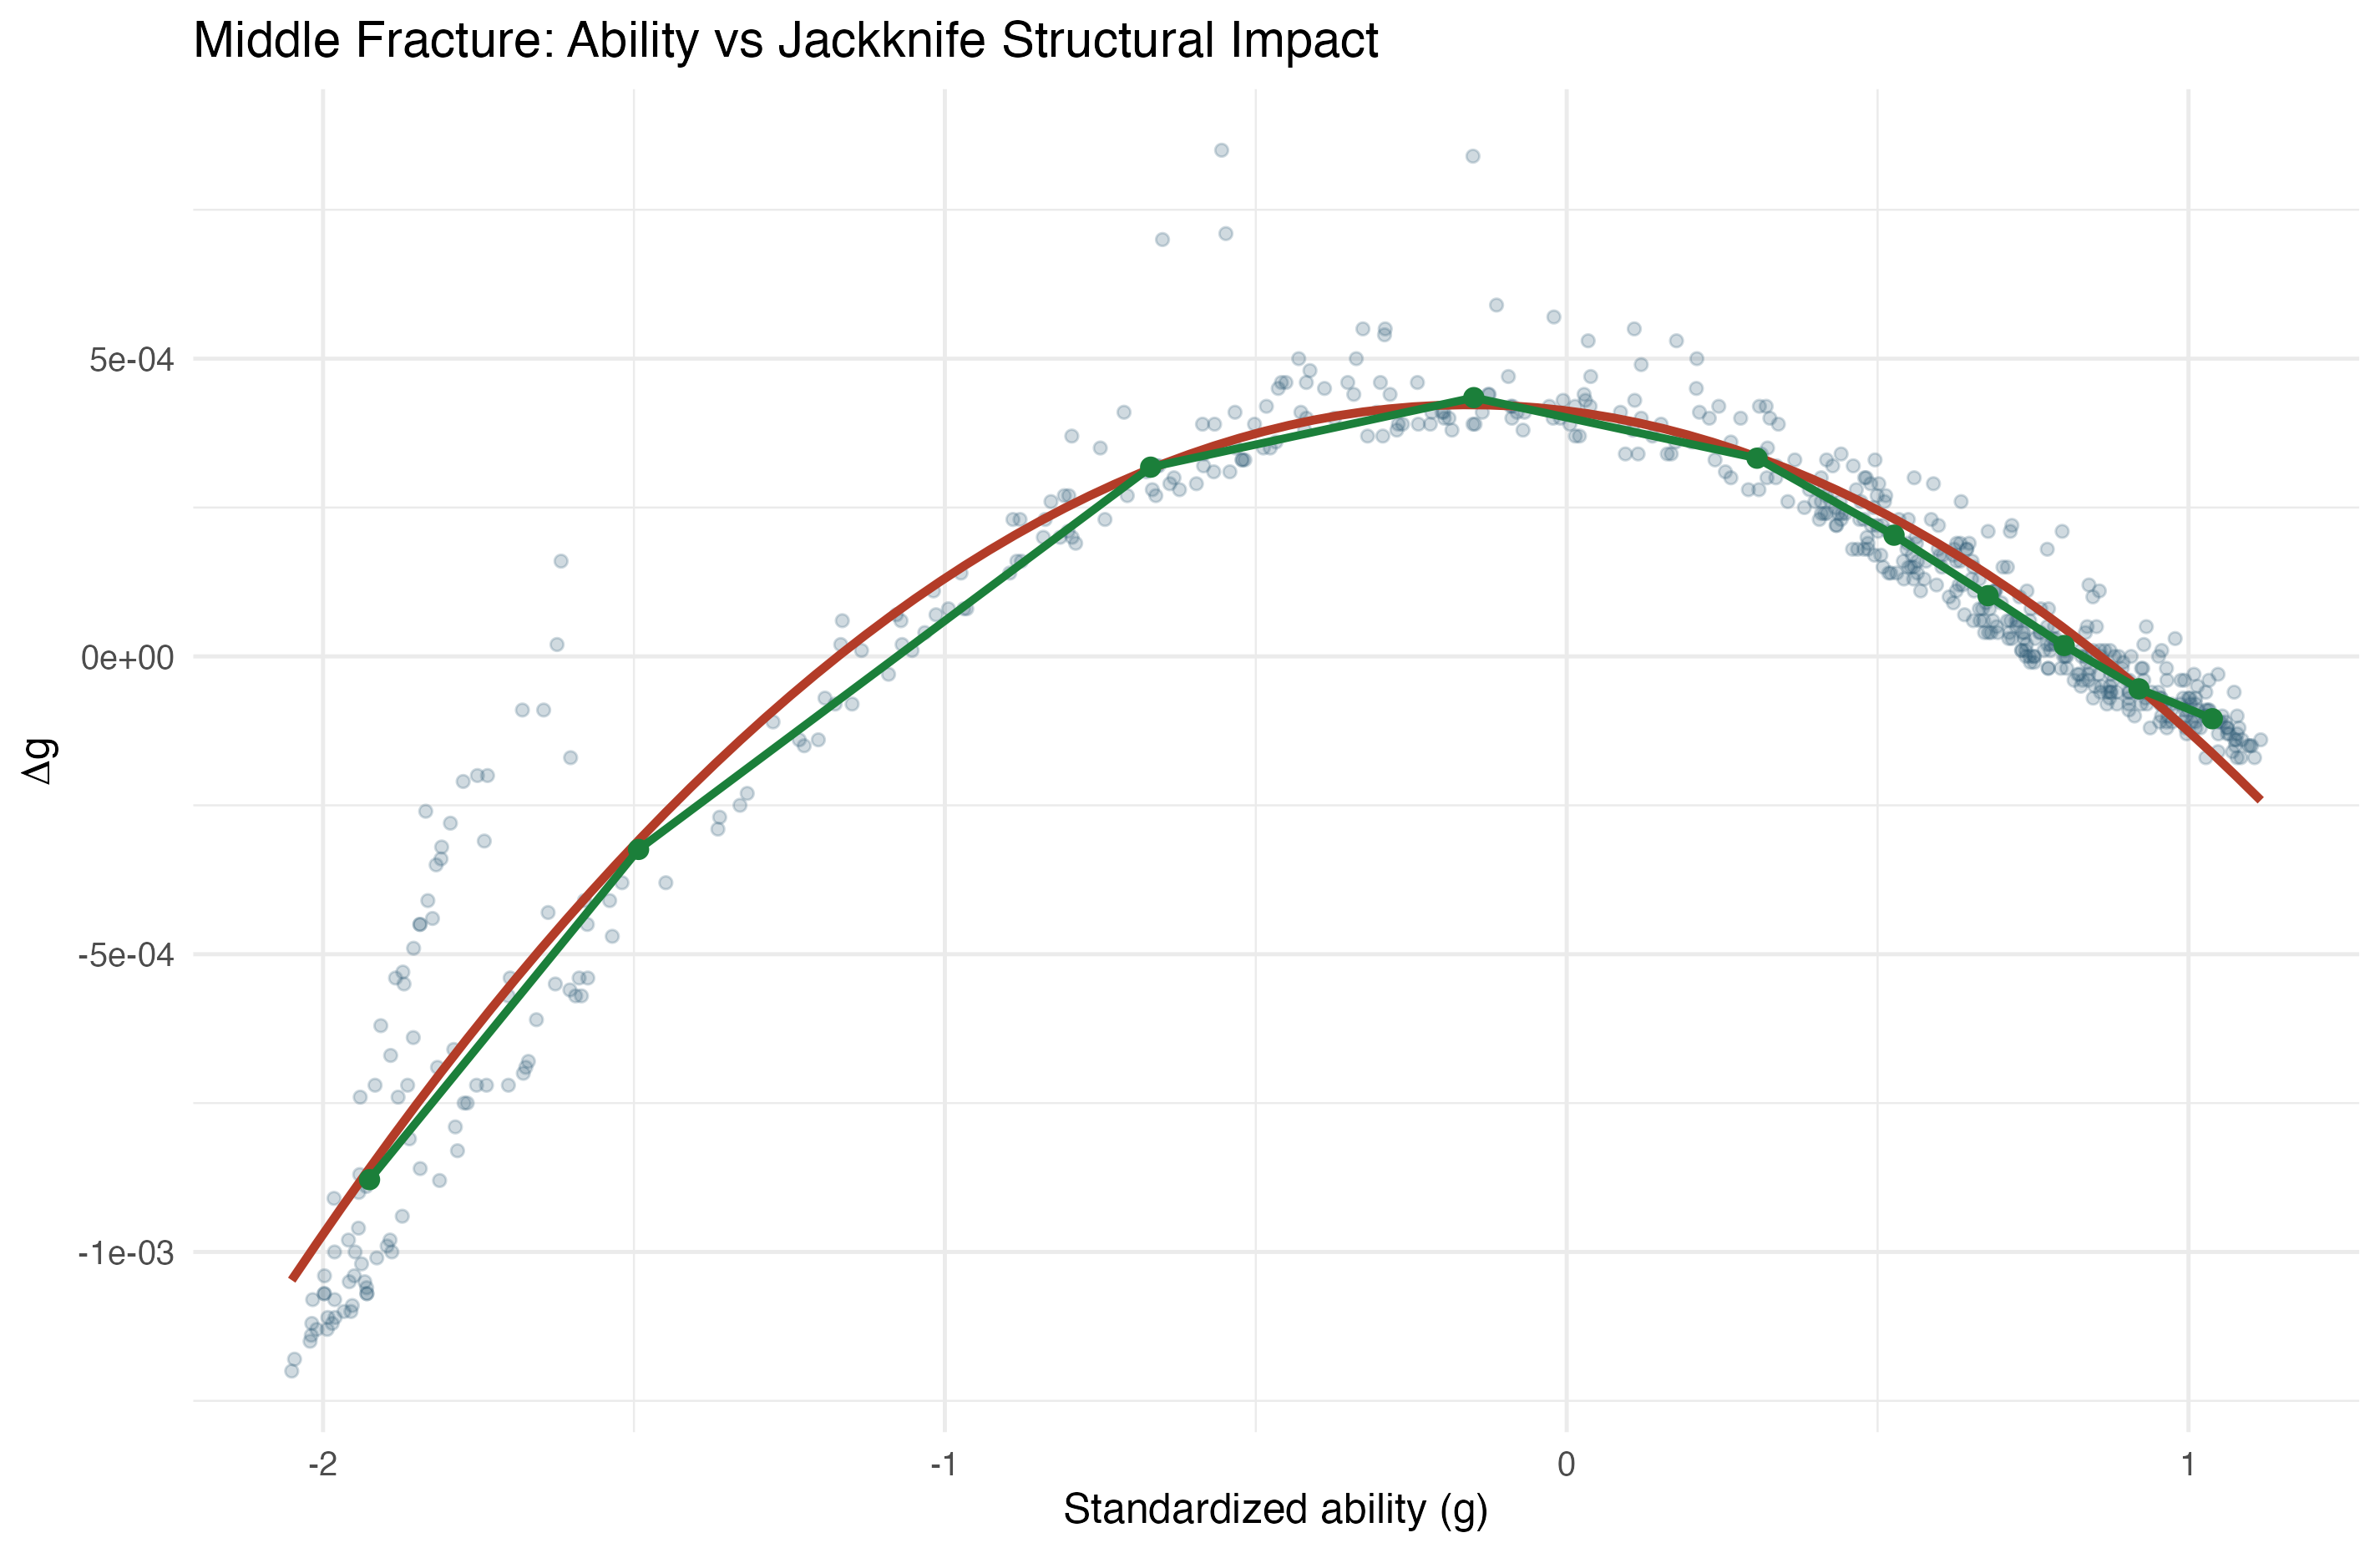
\includegraphics[width=0.94\textwidth]{../outputs/figure_middle_fracture.png}
  \caption{Ability and jackknife structural impact with quadratic fit and decile means. The inverted-U pattern peaks in a middle-ability band and attenuates in the upper tail.}
  \label{fig:middle_fracture}
\end{figure}

Taken together, Figures~\ref{fig:corr_gdelta} and \ref{fig:middle_fracture} should be read differently. Figure~\ref{fig:corr_gdelta} shows why a positive overall correlation is easy to see; Figure~\ref{fig:middle_fracture} shows why that correlation is not the right substantive summary on its own.

\subsection{Regression Tables and Coefficient Interpretation}
Table~\ref{tab:reg_fit_summary} reports fit-level summaries for each model (including bootstrap 95\% CIs for all $R^2$ values and for $g^\star$ under M2). Tables~\ref{tab:reg_linear}--\ref{tab:reg_full} report all regression coefficients with their 95\% confidence intervals.

\begin{table}[H]
\centering
\small
\begin{tabular}{lcc}
\toprule
Model & $R^2$ (bootstrap 95\% CI) & $g^\star$ (bootstrap 95\% CI) \\
\midrule
M1: $\Delta g\sim g$ & $0.294\ [0.222,\,0.362]$ & --- \\
M2: $\Delta g\sim g+g^2$ & $0.927\ [0.908,\,0.945]$ & $-0.157\ [-0.170,\,-0.144]$ \\
M3: $\Delta g\sim g+g^2+\log(1+\mathrm{params})+\mathrm{type}$ & $0.933\ [0.915,\,0.949]$ & --- \\
\bottomrule
\end{tabular}
\caption{Model-level fit summaries and bootstrap percentile intervals ($B=10{,}000$).}
\label{tab:reg_fit_summary}
\end{table}

\begin{table}[H]
\centering
\small
\begin{tabular}{lccc}
\toprule
Term & Estimate & 95\% CI & $p$ \\
\midrule
Intercept & $0.00000327$ & $[-0.0000234,\,0.0000300]$ & $.810$ \\
Ability ($g$) & $0.000213$ & $[0.000186,\,0.000240]$ & $<.001$ \\
\bottomrule
\end{tabular}
\caption{M1 coefficients (linear baseline): $\Delta g=\beta_0+\beta_1 g+\varepsilon$.}
\label{tab:reg_linear}
\end{table}

\begin{table}[H]
\centering
\small
\begin{tabular}{lccc}
\toprule
Term & Estimate & 95\% CI & $p$ \\
\midrule
Intercept & $0.000412$ & $[0.000398,\,0.000427]$ & $<.001$ \\
Ability ($g$) & $-0.000128$ & $[-0.000141,\,-0.000116]$ & $<.001$ \\
Ability$^2$ ($g^2$) & $-0.000410$ & $[-0.000421,\,-0.000399]$ & $<.001$ \\
\bottomrule
\end{tabular}
\caption{M2 coefficients (fracture model): $\Delta g=\beta_0+\beta_1 g+\beta_2 g^2+\varepsilon$.}
\label{tab:reg_quad}
\end{table}

\begin{table}[H]
\centering
\small
\begin{tabular}{lccc}
\toprule
Term & Estimate & 95\% CI & $p$ \\
\midrule
Intercept & $0.000326$ & $[0.000299,\,0.000353]$ & $<.001$ \\
Ability ($g$) & $-0.000167$ & $[-0.000183,\,-0.000151]$ & $<.001$ \\
Ability$^2$ ($g^2$) & $-0.000414$ & $[-0.000425,\,-0.000403]$ & $<.001$ \\
$\log(1+\mathrm{params})$ & $0.0000384$ & $[0.0000277,\,0.0000491]$ & $<.001$ \\
Instruction/chat & $0.0000172$ & $[-0.00000143,\,0.0000359]$ & $.070$ \\
Merge/MoE & $0.0000371$ & $[0.00000857,\,0.0000656]$ & $.011$ \\
\bottomrule
\end{tabular}
\caption{M3 coefficients (controlled quadratic). Category effects are relative to the base/other reference class.}
\label{tab:reg_full}
\end{table}

The coefficient pattern is straightforward. In M1, the positive ability slope reproduces the descriptive tendency for higher-ability models to be more polluting on average, but the model misses the reversal in the upper tail. In M2, $\hat{\beta}_2<0$ defines a concave surface and $m'(g)=\hat{\beta}_1+2\hat{\beta}_2 g$ crosses zero at $g^\star\approx-0.157$, producing the middle-ability peak. The M2/M3 intercepts are evaluated at $g=0$ (the sample mean ability), so they are directly interpretable as predicted structural impact near the center of the observed range. In M3, the ability and curvature terms remain large and stable, so the bifurcation shape is not explained away by size or type controls. The $\log(1+\mathrm{params})$ coefficient is positive, indicating a conditional upward shift in $\Delta g$ at fixed ability and type. The instruction/chat indicator is positive but its 95\% interval crosses zero, so evidence is inconclusive at $\alpha=0.05$. The merge/MoE indicator is positive with a strictly positive 95\% interval, indicating additional pollution relative to base/other models after controlling for ability and size.

\subsection{Popular LLM Families, with Llama in Detail}
The family summaries in Table~\ref{tab:families} show that the global bifurcation is not being driven by a single brand family. Llama is the largest family in the sample ($n=120$) and shows substantial internal spread: high-ability 70B-derived variants are often near-neutral or pillar-like, while several middle-band instruct/merge variants lie in the polluter region. Mistral/Mixtral trends somewhat more pillar-like on average, whereas Gemma and Qwen contain visibly more positive mean structural impact in this snapshot.

\begin{table}[H]
\centering
\small
\begin{tabular}{@{}lrrrrrr@{}}
\toprule
Family & $n$ & Mean $g$ & Max $g$ & Mean $\Delta g$ & Min $\Delta g$ & Max $\Delta g$ \\
\midrule
Llama & 120 & 0.06 & 1.11 & $0.0000614$ & $-0.00113$ & $0.000700$ \\
Mistral/Mixtral & 56 & 0.42 & 1.10 & $-0.0000736$ & $-0.00115$ & $0.000470$ \\
Qwen & 9 & 0.03 & 1.01 & $0.0001940$ & $-0.00005$ & $0.000460$ \\
Gemma & 6 & 0.15 & 0.90 & $0.0003500$ & $-0.00004$ & $0.000500$ \\
DeepSeek & 10 & -0.17 & 1.06 & $0.0000590$ & $-0.00056$ & $0.000550$ \\
\bottomrule
\end{tabular}
\caption{Family-level summary for popular open model lines in this snapshot. Means are informative, but the main message is the substantial within-family spread.}
\label{tab:families}
\end{table}

Within Llama, tercile analysis is particularly informative. The low-ability tercile has mean $\Delta g\approx-0.0000768$, the middle tercile has the largest positive influence (mean $\Delta g \approx 0.000239$), and the upper tercile returns close to zero (mean $\Delta g \approx 0.0000223$). This pattern aligns with the global bifurcation and argues against treating ``Llama'' as a psychometrically homogeneous category.

Representative Llama polluters in the snapshot include yayi2-30B-Llama, Telugu-Llama-7B-Instruct, and Guanaco-Unchained-Llama-2-7B, whereas representative high-ability Llama pillars include Grafted-Llama2-2x70B and related 70B-class derivatives with negative $\Delta g$.

\section{Discussion}
The central empirical result of this psychometric audit is that the latent-structure alignment tax is not well described as a single monotonic slope. In this snapshot, structural pollution rises into a middle-ability band and then attenuates in the upper tail. That is why the paper argues for capacity-conditioned bifurcation rather than uniform degradation. The claim is geometric rather than rhetorical: the same benchmark ecosystem can simultaneously retain a dominant general factor and exhibit model-specific perturbations of that factor.

This framing complements recent LLM evaluation work that treats item calibration and benchmark design as measurement problems rather than mere leaderboard engineering. Factor-analytic studies show that common variance can be substantial while still leaving meaningful residual structure \citep{burnell2023structure, ilic2024interrelated}. IRT-style benchmark audits, adaptive testing papers, and data-efficient evaluation frameworks likewise show that ability estimates depend on item properties, item selection, and the measurement model used to summarize performance \citep{zhou2026lost, tambon2025taskeval, taschetto2025enem, truong2025amortized, li2026adaptive, liao2025legoirt, chen2025irtnet, hofmann2025fluid, krumdick2026abilities, xu2025lart}. The present article adds a complementary question to that literature: not only which items are informative, but which models distort or stabilize the shared latent structure of the benchmark matrix itself.

The practical implication is modest but important. Leaderboard gains and latent-structure gains should be treated as related but non-identical quantities. A model can look strong in aggregate and still be psychometrically disruptive relative to the dominant factor geometry, especially in the middle of the ability range. Conversely, the high-ability tail in this snapshot contains several models that are near-neutral or pillar-like under jackknife deletion. For benchmark interpretation, that means aggregate rank should not be assumed to exhaust what has changed when a model improves.

Recent work on contamination-aware benchmarking and psychometric leaderboard redesign makes the same broader point from neighboring angles: score validity depends on the properties of the benchmark, the items, and the summary statistic used to report performance \citep{wu2025antileakbench, chen2025emnlpcontam, chen2025recentcontam, federiakin2025leaderboards}. The present results fit naturally within that emerging view, while focusing specifically on latent-structure cohesion in an ultra-wide model-by-item matrix.

\section{Limitations}
First, this study is a fixed historical audit and does not include updated post-2024 leaderboard data. The ecosystem has changed substantially since April 8, 2024, so direct extrapolation to current frontier models is not warranted. The present manuscript therefore supports a claim about the analyzed snapshot, not a universal law of all future LLM generations.

Second, the response matrix is binary and sparse in semantic richness. Binary correctness is useful for psychometric factor extraction, but it cannot by itself distinguish calibration quality, instruction-following style, safety policy effects, or reward-model overfitting pathways. Some apparent structural effects may thus bundle multiple latent causes.

Third, the jackknife criterion is tied to first-factor variance concentration. While this is interpretable, it is still a model-based structural criterion and not a causal estimate of training interventions. A positive $\Delta g$ does not prove intentional gaming; it indicates incompatibility with the dominant latent geometry under this particular measurement model.

Fourth, model-family and training-type labels are inferred from repository names. This is unavoidable in large open snapshots, but it introduces classification error. Family-level comparisons should therefore be treated as robust descriptive summaries, not as definitive taxonomies.

Fifth, closed-source frontier models are absent, and open-source publication bias may distort the observed ability-fracture surface. A complete ecosystem claim would require harmonized item-level data for both open and proprietary systems.

Finally, this manuscript operationalizes the latent-structure alignment tax with a single structural criterion ($\Delta g$). Future work should triangulate this jackknife criterion with explicit IRT latent-trait diagnostics and item-difficulty modeling \citep{wu2020virt, cai2010highdim, chalmers2012mirt, li2025itemdifficulty, scarlatos2025smart}. Recent adaptive-evaluation frameworks suggest that such calibrated latent-trait approaches can also support much more efficient benchmark design \citep{truong2025amortized, zhou2026lost, li2026adaptive, liao2025legoirt, hofmann2025fluid, krumdick2026abilities, xu2025lart}.

\section{Conclusion}
The audited snapshot supports two claims at once. First, the open-weight benchmark matrix retains a strong general factor. Second, structural impact is not a simple monotonic function of ability: it peaks in a middle-ability regime and attenuates at the high-ability tail. In that sense, this psychometric audit of open LLM benchmarks supports a capacity-conditioned, not uniform, account of the latent-structure alignment tax.

\bibliographystyle{plainnat}
\bibliography{references}

\end{document}
